%!TEX root = ../thesis_a4.tex

\chapter{Introduction}
\label{sec:intro}

\section{Motivation}
\label{sec:intro:motivation}

Information sharing is considered by some authors as being an ``attribute of humanity itself''~\citep{Dunbar1996,Rafaeli2005}.
In the last two decades, the web has revolutionized the way in which information is shared among human beings.
The so called \emph{social media} revolution~\citep{Smith2009} has brought sharing to a whole new level. 
%Notably, some consider that information sharing is an ``attribute of humanity itself''~\citep{Dunbar1996,Rafaeli2005}.
Nowadays, all kinds of information such as books, articles, opinions, videos, pictures and audio tracks are hosted in online sharing platforms accessed by millions of users worldwide.
Besides the fact that the amount of information that is accessible through the internet is huge, far bigger than what was available through traditional channels (i.e.,~libraries, television, radio, shops, etc.), there is something very particular in the online sharing paradigm:
much of the content that is shared online is generated by the users of these sharing platforms~\citep{Kietzmann2011}, the so called \emph{user generated content}~\citep{Kaplan2010}.
%\TODO{motivations that user have to share this content are very different than traditional industry motivations, \citep{Daugherty2008,Katz1960}}
% User generated content: this term ``is usually applied to describe the various forms of media content that are publicly available and created by end-users'' \citep{Kaplan2010}.
%\citep{Daugherty2008,Katz1960} one of the reasons for sharing user generated content- ``In contrast, 
%the knowledge function recognizes that people are driven by 
%the need to gain information to organize and understand their 
%environment. That is, we are motivated by the need to 
%understand and make sense of our experiences''

Such user generated content potentially represents an incredibly valuable resource that can serve several purposes, ranging from business and research applications to artistic creation and the preservation of cultural heritage~\citep{Krumm2008}. 
Nevertheless, the value of user generated content is significantly dimmed by the ways in which such content can be accessed and reused.
As the amount of content grows, so does the difficulty of browsing and locating what one needs, and so do the challenges that search engines have to face.%\cite{Woods1999} data availability paradox

For the content to be accessible, it needs to be properly indexed.
However, the quantity and variety of user generated content turns proper indexing into a very difficult task. 
This is particularly true for multimedia resources like video, pictures and audio -- typically the most popular in the user generated content world -- which, as opposed to other kinds of media, do not have a direct textual representation~\citep{Bischoff2008}. 
Moreover, as user generated content does not normally follow a traditional editorial process before publication, no standard metadata is generated that can help the indexing process.
At the same time, the amount of content generated is simply too much to be curated in scalable ways by groups of experts~\citep{Mathes2004}.

Online sharing platforms typically delegate the responsibility of describing or annotating\footnote{In this thesis, the terms ``annotation'' and ``description'' can both be used interchangeably, and may refer to all kinds of metadata that can accompany an online resource.} their content to the users, that is to say, the \emph{authors} or \emph{contributors}. Thus, content description is done in a distributed fashion.
The nature of content annotations may vary depending on each particular sharing platform, and is highly dependent on the description mechanism used in every particular site.
Description mechanisms that look for the most uniform annotations can use forms with a number of predefined fields with fixed responses that users need to choose from when uploading a resource. For example, users might be asked to select a music genre from a particular list when uploading an audio track to an audio sharing platform.
However, these mechanisms lack flexibility when new resources are uploaded, as their characteristics can be unexpected and not contemplated in the description form~\citep{Mathes2004,shirky2005ontology,halpin2006,Macgregor2004}. Other description mechanisms provide more flexibility by not limiting form fields to a specific set of responses. In that case, annotations typically consist of a textual description plus a list of labels assigned by the users which are not restricted to a particular vocabulary.
These labels are commonly known as \emph{tags}, and act as keywords that describe the content.
In both cases, users may apply their own ideas and rationale to decide how to describe the content, working at different levels of abstraction, and understanding the goal of the annotation process in different ways~\citep{golder2006}. 
If we were to ask two different users to independently annotate a single online resource, we would most probably find little overlap in their responses. This illustrates the so called \emph{vocabulary problem}~\citep{Furnas1987}, which clearly shows up in today's online sharing platforms~\citep{marlow2006}.
%Hence, uniformity of content descriptions is a rare property in online sharing sites. 

Consequently, the organisation, browsing and searching capabilities of online sharing platforms is rather limited, particularly of those focused on multimedia sharing. 
For example, in YouTube\footnote{\url{http://www.youtube.com}. All URLs in this thesis were last accessed on 11 March 2015.}, SoundCloud\footnote{\url{http://www.soundcloud.com}.} or Flickr\footnote{\url{http://www.flickr.com}.} (well known sites for sharing video, music and photos, respectively), the main way of accessing content is by introducing some textual query terms to be matched against resources' metadata (i.e.,~filenames, textual descriptions, tags, etc.). In some cases, search results can be filtered using basic file properties (i.e.,~duration, size, data format, etc.) and simple metadata (i.e.,~upload date, license, geolocation, etc.), or augmented through automatic resource recommendation systems and information from social connections (i.e.,~friends, followed users, etc.). YouTube and SoundCloud also offer the option to filter content using a number of predefined categories for kinds of videos and music genres, respectively. These categories can be filled in by users when describing their content during the upload process.
However, no comprehensive faceted or hierarchical browsing functionalities are possible, and no advanced search filters can be defined that can operate at a higher semantic level. For example, it would be desirable to reliably filter resources according to objects appearing in pictures or videos, or musical instruments in audio tracks.

In order to mitigate the annotation problems, substantial research has been conducted to derive computational methods for automatically annotating multimedia resources. These methods are based on the analysis of resources's content, that is to say, pixel values in pictures and video, and the audio waveform in sound and music. For example, methods have been proposed for recognizing semantic concepts in pictures~\citep{Li2006}, for identifying human actions in videos~\citep{Poppe2010}, for automatically classifying audio tracks in musical genres~\citep{Scaringella2006} or for the identification of environmental sounds~\citep{Chachada2013}.
Some of these methods can achieve reasonably high accuracies and potentially allow for a uniform annotation of resources without the need of user intervention. However, these are generally still far from satisfactory in real-world scenarios~\citep{Wang2012}.

It is the rationale of this thesis that if we concentrate on acquiring better content annotations from the authors themselves, we can obtain more accurate descriptions at higher semantic levels that could hardly be obtained otherwise using current content-based approaches. 
%Furthermore, these descriptions can then be used to train content-based models to automatically describe some characteristics of unannotated media resources.
Hence, the idea of focusing on the acquisition of better annotations from users that upload content to online sharing sites is the starting point of our work. 
In particular, in this thesis we propose methods aimed at the improvement of tag annotations of user generated content.

%The idea of focusing on the acquisition of better annotations from users that upload content to online sharing sites, is the starting point of our work. In this thesis, we particularly work on the domain of sound and music, and propose methods aimed to the improvement of the annotations of user generated content.
%The methods we propose, as well as their impact, are thorougly evaluated in the context of an online sound sharing site with more than 215,000 uploaded resources and almost 4 million registered users. 


\section{Tagging systems and folksonomies}
\label{sec:intro_tagging_systems_and_folksonomies}

% Predecessors de tagging systems anomenats a \cite{Sen}, primera pàgina: pharos, knowledge pump, fab

Using tags as keywords for annotating resources has become standard practice in online sharing sites.
Tags, as a common form of user provided metadata, were first introduced in the bookmark sharing site Delicious\footnote{\url{http://www.delicious.com}.}~\citep{Gupta2010, wikipedia_tag}, and have been adopted by many other sites. To name a few examples, sites that incorporate tagging systems include Flickr (photo sharing), YouTube and Vimeo\footnote{\url{http://www.vimeo.com}.} (video sharing), CiteULike\footnote{\url{http://www.citeulike.org}.} and Mendeley\footnote{\url{http://www.mendeley.com}.} (for sharing scholarly references), SoundCloud, Last.fm\footnote{\url{http://www.last.fm}.} and Freesound\footnote{\url{http://www.freesound.org}.} (audio and music sharing), StackExchange\footnote{\url{http://www.stackexchange.com}.} (question and answer sites), and Blogger\footnote{\url{http://www.blogger.com}.} and Wordpress\footnote{\url{http://www.wordpress.org}.} (blogging sites).

\begin{figure}[t]
  \centering
  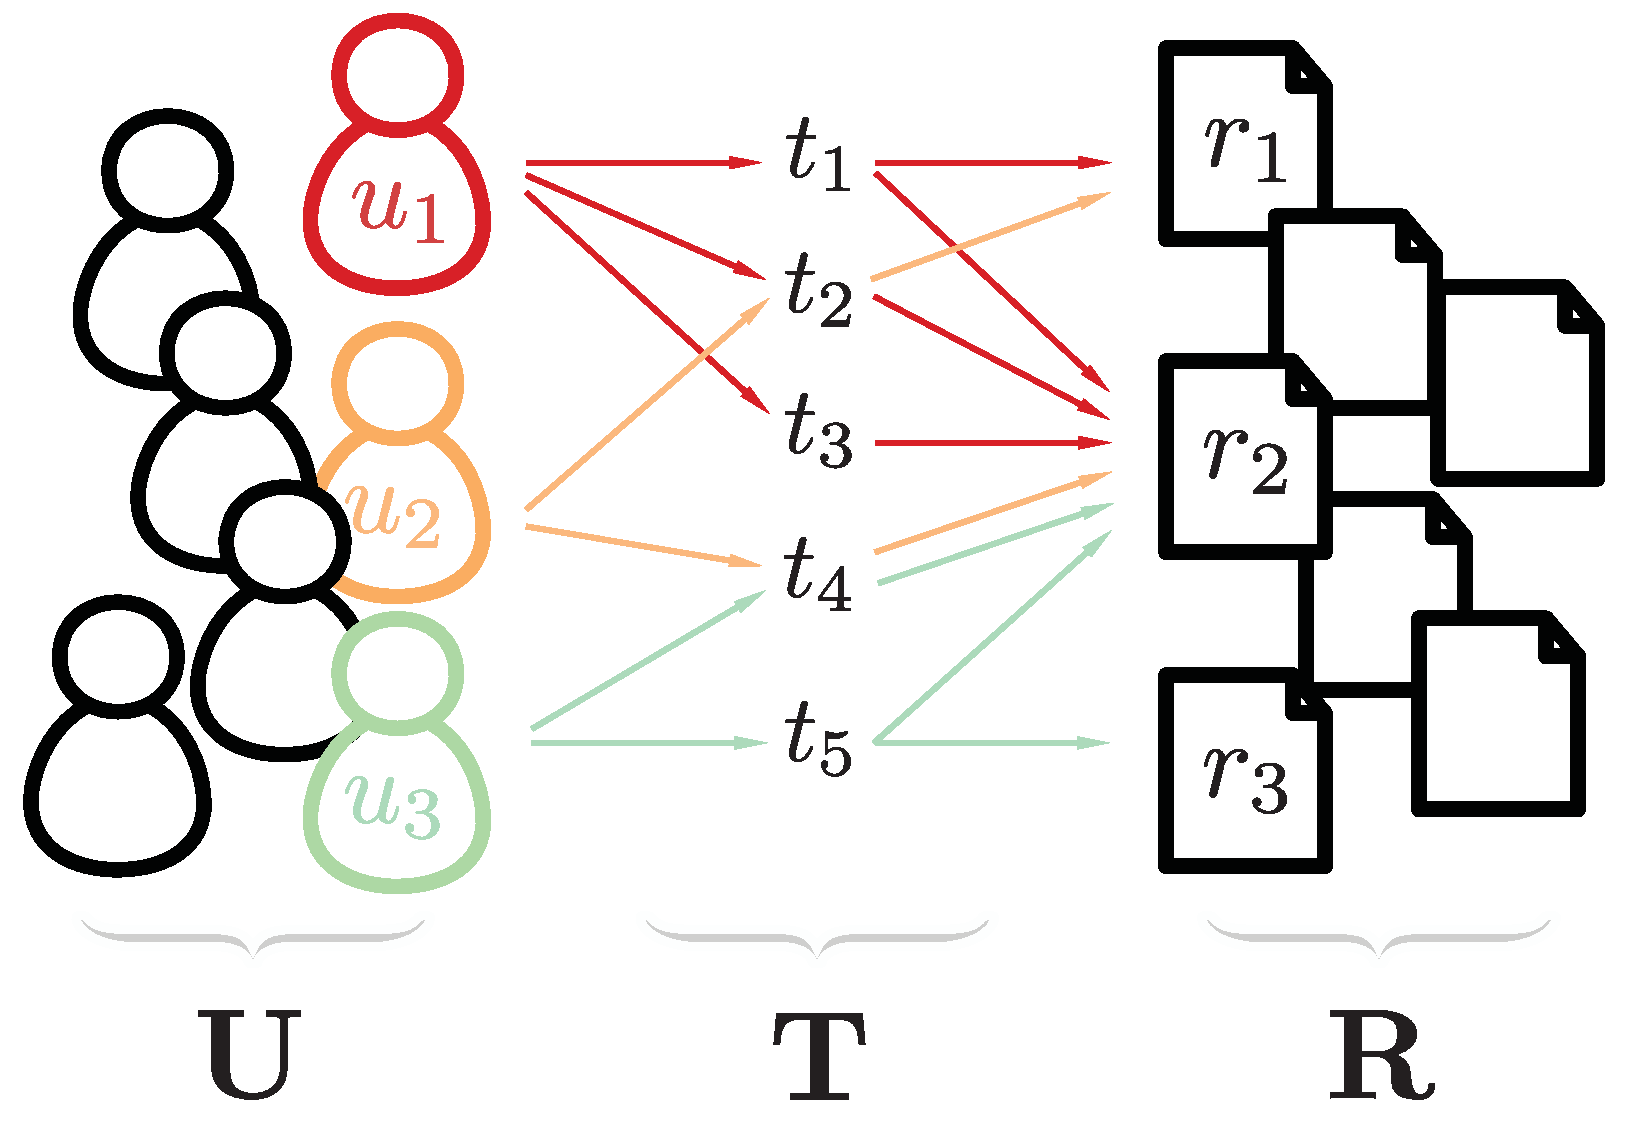
\includegraphics[width=0.7\textwidth]{ch01_introduction/pics/tagging_diagram}
  \caption[Conceptual diagram of tagging systems]{Conceptual diagram of tagging systems. $\users$, $\tags$ and $\resources$ correspond to a set of users, tags and resources, respectively, while $\user_i$, $\tagb_i$ and $\resource_i$ correspond to individual users, tags and resources.}
  \label{fig:tagging_diagram}
\end{figure}

Tags are free-form textual labels that convey some semantically meaningful information about the content resource to which they are assigned. Users apply these labels to content resources, hence \emph{tagging} is the action that a user performs when assigning a tag to a resource\footnote{In this thesis we also use the terms ``tagger'' or ``annotator'' to refer to a user that assigns tags to a resource.}. In Fig.~\ref{fig:tagging_diagram}, we show a conceptual diagram for tagging systems. In it, we can observe that every tag $\tag \in \tags$ can be related with a number of users $\user \in \users$ and resources $\resource \in \resources$. Every unique tag-user-resource ternary relation (e.g.,~the path that relates $\tag_1$, $\user_1$ and $\resource_1$ in Fig.~\ref{fig:tagging_diagram}), is known as a \emph{tag application}~\citep{Sen}. In this thesis, we will refer to the union of all tags related to a particular resource as the resource's \emph{tagline}. In the example of Fig.~\ref{fig:tagging_diagram}, the tagline of $\resource_1$ corresponds to $\{ \tag_1, \tag_2 \}$, whereas the tagline of $\resource_2$ corresponds to $\{ \tag_1, \tag_2, \tag_3, \tag_4, \tag_5 \}$.
%Conversely, the union of all tags related to a particular user is generally known as the user vocabulary.

The aggregate of all tag applications which relate the tags, users and resources of a sharing site, is commonly known as a \emph{folksonomy}~\citep{Wal2007Folksonomy}. This term has been extensively used in the tagging systems literature, not only to designate the set of tags, users, resources and ternary relations of a sharing site, but also to refer to the implicit information and knowledge embedded in this space. However, its original meaning, as introduced by~\cite{Wal2007Folksonomy}, is somewhat more restrictive and particularly refers to those tagging systems in which tag applications are made by the consumers of online resources, not necessarily the authors of the content (see below). 
In folksonomies, unlike more rigid structures such as taxonomies or ontologies, the semantic terms represented by tags are organized without hierarchy, and are a close representation of the vocabulary of the users in an online sharing platform~\citep{Gupta2010}. In fact, the set of tags of a folksonomy is commonly known as the \emph{vocabulary} of the folksnonomy or of a tagging system.
%Vander Wal on folksonomy: ``Folksonomy is the result of personal free tagging of information and objects (anything with a URL) for one's own retrieval. The tagging is done in a social environment (shared and open to others). The act of tagging is done by the person consuming the information.''

There are several types of tagging systems which differ in their design and purpose. Generally, the types of content resources that are shared bring some important implications regarding the design of tagging systems. On the one hand, in those sites in which users share \emph{references} to already existing resources (e.g.,~links to web pages), tags are typically added by the users that consume these resources to allow further easy retrieval. As a result, a single resource can be tagged by many users, and a single tag can be assigned more than once to the same resource. The folksonomy resulting in tagging systems of this type is called a \emph{broad folksonomy}~\citep{Wal2007BroadNarrow}, and is the one that is more closely related to the original definition of folksonomy. Delicious, Last.fm  and CiteULike are examples of online sharing sites featuring broad folksonomies. 
On the other hand, in sites where user generated content is shared, tags are typically assigned by the authors of the resources (i.e.,~the users that upload the resources) so that these are accessible to other users~\citep{Cattuto2006}. In that case, the resulting folksonomy is called a \emph{narrow folksonomy}~\citep{Wal2007BroadNarrow}, and tags are only assigned once to particular resources. Examples of tagging systems with narrow folksonomies include multimedia sharing sites like Flickr, YouTube, Soundcloud and Freesound.

In the tagging systems literature, it is very common to use the terms \emph{social tagging} and \emph{collaborative tagging} to refer to tagging systems in general. Although the terms are normally treated as being exchangeable, their original meanings have some implications. 
The term collaborative tagging, first introduced by~\cite{golder2006}, specially refers to these tagging systems in which resources can be tagged by any user (not only the authors), thus resulting in broad folksonomies. 
The term social tagging, introduced by~\cite{marlow2006}, refers to sharing sites in which tags are  particularly exposed to consumers and shared among contributors, and not only used for the self organisation of contributors' resources. In this thesis, we employ the more generic term ``tagging systems''.
The annotation of resources using tagging systems allows online sharing platforms to provide a number of functionalities for indexing, searching and browsing their content. For example, using a \emph{tagcloud} (Fig.~\ref{fig:tagcloud}), users can have an idea of the most popular tags used in a tagging system and navigate among resources by filtering their tags.
\begin{figure}[t]
  \centering
  \includegraphics[width=0.72\textwidth]{ch01_introduction/pics/flickr_tagcloud}
  \caption[Flickr tagcloud]{Flickr tagcloud (as retrieved on 24 July 2014).}
  \label{fig:tagcloud}
\end{figure}
In a way, the folksonomy can be used as a ``semantic map'' to navigate the contents of a sharing site~\citep{Cattuto2006}.

Despite the popularity of tagging systems and their successful implementation in many online sharing sites, there are a number of well-known problems which limit the possibilities of these functionalities~\citep{Guy2006}.
These problems range from the use of different tags to refer to a single concept (synonymy) and the ambiguity in the meaning of certain tags (polysemy), to tag scarcity and the appearance of typographical errors~\citep{golder2006,halpin2006}. 
Furthermore, the quality of the indexing, searching and browsing functionalities enabled by tagging systems strongly relies on the coherence and comprehensiveness of the tags assigned to the resources.
This does not only apply at the scope of a particular tagline of a resource, but also at the scope of the whole folksonomy~\citep{Spiteri2006}.
In other words, it is not only important that individual resources are properly tagged, but also that there is a coherence across the descriptions of all resources in the folksonomy.
For that reason, it has been often discussed whether the folksonomy of a tagging system, after a certain time of being in use, reaches a point of implicit consensus where the vocabulary converges to a certain set of tags and tagging conventions that are widely adopted by all users of the system~\citep{halpin2006,Sen,Sood2007,Robu2009,Wagner2014}.
According to these authors, the point of consensus may be reached because of imitation patterns and users' shared cultural knowledge.
Reaching that point of consensus is desirable to improve the browsing and searching experience of a site~\citep{Guy2006}.

For addressing some of the aforementioned problems of folksonomies, the literature of tagging systems has often proposed the implementation of tag recommendation methods to aid users in the tagging process~\citep{golder2006,halpin2006,marlow2006}. 
By using such methods, user annotations are expected to be more uniform and comprehensive.
The study of tag recommendation systems is the main topic of this thesis.

%``thoughtful sociotechnical design of tagging systems may uncover ways to overcome the Vocabulary Problem without requiring either the rigidity and steep learning curve of tightly controlled vocabularies, or the computational complexity and relatively low success of purely automatic approaches'' \cite{marlow2006}


\section{Tag recommendation}

Tag recommendation systems are used to suggest potentially relevant tags to users when they are annotating online resources. In this way, tag recommendation assists users during the annotation process, and can have a considerable impact on the resulting annotations and folksonomies. 
Depending on the type of information that a tag recommendation system employs when suggesting tags, systems can be generally categorized into three main groups~\citep{Wang2012}:
\begin{itemize}
\item The first group  corresponds to the systems that, given a user $\user$ annotating a resource $\resource$, analyse the content of the resource $\resource$ and automatically extract a number of features that can be related to a set of tags $\recommendedTags$ which are finally recommended. 
For example, given an image file, an automatic system could be used to try to automatically recognize an object appearing in the image and then the name of that object could be suggested to the user as a tag. We refer to these kind of systems as content-based tag recommendation systems.

\item The second group corresponds to the systems that, to generate $\recommendedTags$, take into account the folksonomy of the tagging system and a set of tags $\inputTags$ that have already been assigned to the resource $\resource$. In that case, the system could recommend tags that are popular or that have been frequently used alongside the tags in $\inputTags$. These systems are known as folksonomy-based tag recommendation systems.

\item The third group includes recommendation systems which rely on other types of metadata and contextual information to generate the recommendations. Such systems would, for example, use the title of a resource or any associated geolocation metadata to query an external service like a search engine and extract some keywords from the results to generate $\recommendedTags$. We refer to these kind of systems as context-based tag recommendation systems.
\end{itemize}

In some cases, tag recommendation systems incorporate sources of information belonging to more than one group.
For example, a tag recommendation system can combine content analysis and folksonomy information to generate a list of tag suggestions.
The diagram in Fig.~\ref{fig:tag_recommendation_diagram} illustrates the concept of tag recommendation and the different kinds of information sources that can be used in recommendation algorithms.


\begin{figure}[t]
  \centering
  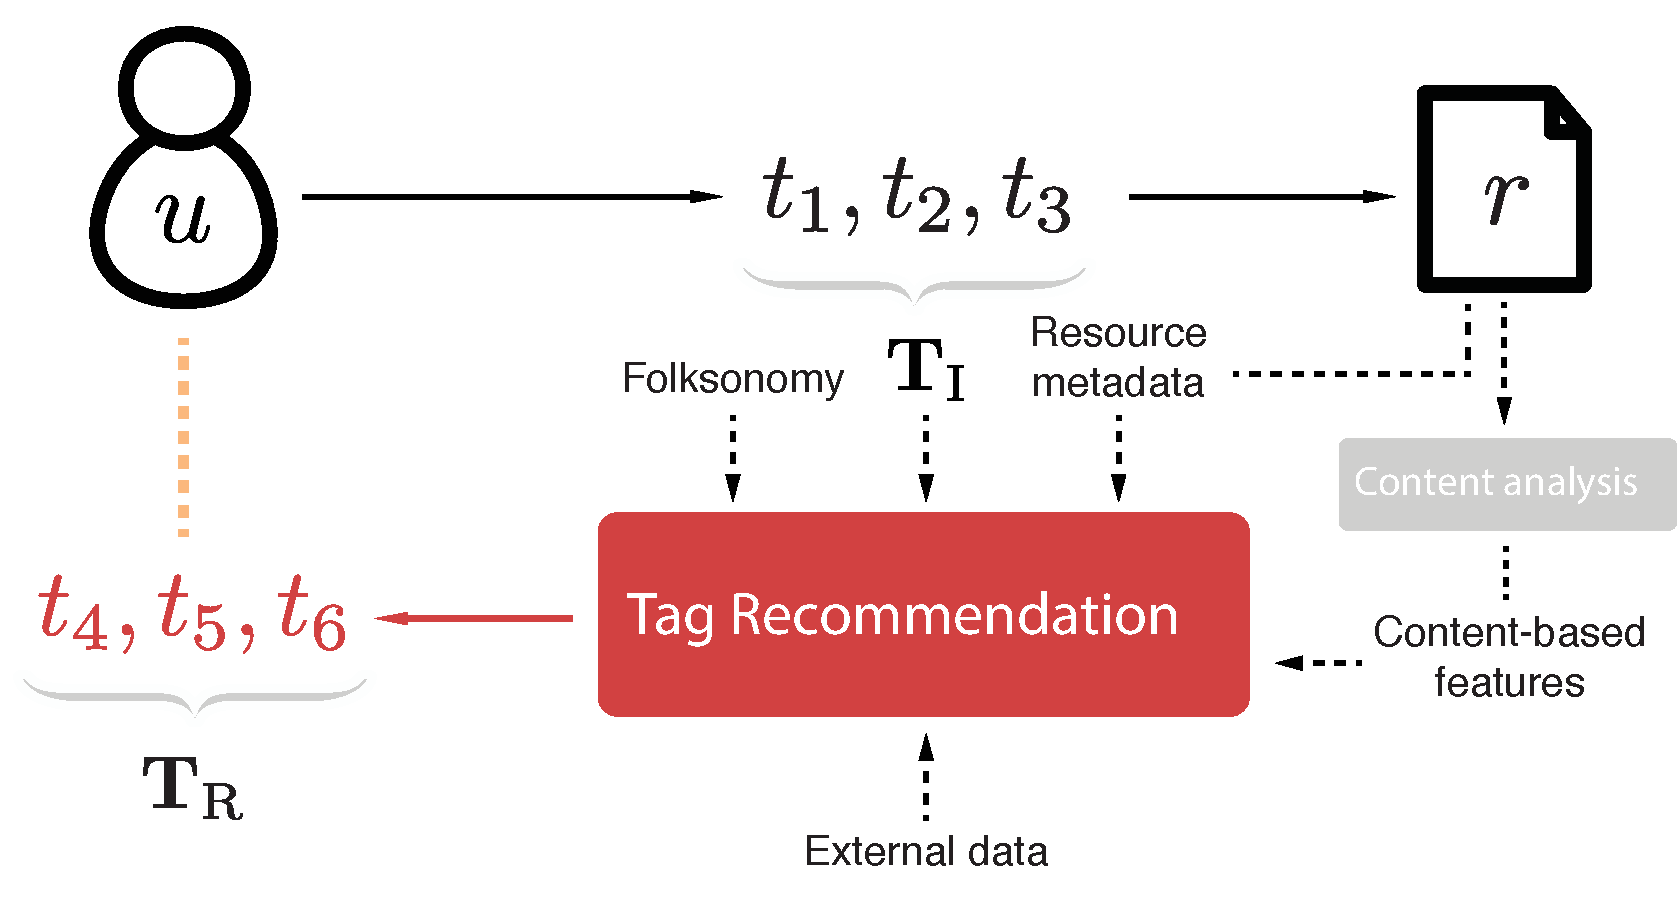
\includegraphics[width=0.8\textwidth]{ch01_introduction/pics/tagging_recommendation_diagram}
  \caption[Conceptual diagram of tag recommendation systems]{Conceptual diagram of tag recommendation systems. $\recommendedTags$ corresponds to a set of recommended tags, while $\inputTags$ corresponds to a set of input tags. Similarly to Fig.~\ref{fig:tagging_diagram}, $\user$, $\tagb$ and $\resource$ correspond to individual users, tags and resources, respectively.}
  \label{fig:tag_recommendation_diagram}
\end{figure}
An important advantage of content-based tag recommendation systems is that they can generate tag recommendations for resources that do not have any kind of metadata. Conversely, folksonomy-based tag recommendation requires the existence of at least one tag assigned to a resource $\resource$ in order to generate recommendations tailored to that particular resource $\resource$, and context-based tag recommendation systems also require at least a partial annotation of the resources in order to provide tag suggestions.
Nevertheless, folksonomy-based and context-based tag recommendation systems have the advantage of not requiring any specific processing of the content of resources being annotated, thus typically being less computationally expensive and more easily generalisable to other types of resources.
Among the different types of tag recommendation systems described above, this thesis is focused on those based on the analysis of the folksonomy of a tagging system.

%\point State what kind of approach we do follow, with which current approaches it is related, and which ``gaps'' are we trying to cover (just briefly, it will be treated in more detail in ``Objectives and outline of the thesis'', at the end of this section).

Once a tag recommendation system generates a set of recommended tags $\recommendedTags$ for a resource $\resource$, these are normally presented as a suggestion to the user that is annotating $\resource$. Users can then decide whether or not to add any of the tags in $\recommendedTags$ as an annotation of $\resource$. Hence, the user acts as a judge for the quality and appropriateness of the recommendations.
Intuitively, a good tag recommendation system suggests tags that users tend to consider as appropriate and therefore are added to the resource tagline. However, besides suggesting relevant tags, tag recommendation systems can also bring other benefits to the annotation process. Even when suggested tags are not considered relevant, these may inspire or convey the sorts of information that users should annotate~\citep{Ames2007}. For example, when annotating a music track, a tag recommendation system could recommend a tag that describes a music genre like \atag{pop}. This tag might not be relevant for the particular music track, but it might remind the user to add a tag describing the correct genre.
Moreover, tag recommendations can be useful to promote the use of a particular form of a concept (e.g.,~suggesting the tag \atag{street-music} instead of \atag{streetmusic}), to prevent misspellings when introducing tags and, in general, to facilitate the tagging process~\citep{Sood2007,jaske2007,Wang2012}.
As a result, many authors hypothesize that tag recommendation systems have a positive impact on the folksonomy of a tagging system, improving the quality of resource annotations~\citep{Jaschke2012,Wang2012} and the coherence and convergence of the vocabulary of the folksonomy~\citep{golder2006,marlow2006,jaske2007,Sood2007,Zangerle2011}. 
This is also one of the aspects that we investigate in this thesis.

Nevertheless, we would like to point out that tag recommendation systems could also be expected to have a negative impact on the folksonomy of a tagging system. Even though we are not aware of such claims in the tagging literature, we could hypothesize that an excess of homogenisation in resource annotations would result in a loss of their informational value, making it hard to distinguish among resources just by looking at their annotations. 
However, considering that non-uniformity of resource annotations is typically listed as an important issue of tagging systems~\citep{Spiteri2006}, the degree of homogenisation that would be required in order to effectively reduce informational value seems intuitively far from its current state.
As another possible negative aspect, it could be argued that providing tag suggestions could make it easier for users to poorly annotate their content by, for example, randomly choosing tags from the list of recommendations. Nonetheless, this kind of resource annotations could also be performed without the use of a tag recommendation system. Hence, this potential problem seems to be more related with the motivations that users have when annotating content (see~\ref{soa:user_motivations}).
For all these reasons, in this thesis we do not evaluate the hypothetical negative impact of tag recommendation systems. 

%``Second, the suggested tags, even when not selected, inspired some participants to add their own tags and gave them direction as to the sorts of tags they should use (e.g., seeing other neighborhood names as suggested tags could encourage the user to add a tag for their neighborhood as well).'' -> from \cite{Ames2007}


\section{Online multimedia sharing}

Multimedia sharing is one of the areas in which the social web has experienced the biggest and quickest growth~\citep{Smith2009}. It can be roughly divided into video, image and audio sharing.
Just to name a few examples, in every minute, 100 hours of video are uploaded to YouTube~\citep{TheYouTubeTeam2013}, 2,400 photos are uploaded to Flickr~\citep{Jeffries2013}, and 12 hours of music are uploaded to SoundCloud~\citep{Wahlforss2013}. %Some of these content resources could be later transformed, remixed, combined, mashed-up and probably reuploaded to online sharing sites in the form of new creations.
The intent with which users upload and share multimedia content can vary widely, but we can identify some general patters according to the usage that the uploaders may expect of the contributed content. On the one side, we can identify those contents that are meant to be accessed and consumed through the online sharing platform itself. In that case, users might upload a photo, a video or a music track and expect other users to consume it \emph{in-place}. Hence, the \emph{end use} of the resource is its online consumption. For example, someone may upload photos of an event to a photo sharing site so that other participants of that event can have access to the photos, or a musical artist can upload a music album to a music sharing site so that other users can listen to it.
On the other side, there is an additional type of uploaded content which is meant to be reused outside the sharing platform where it is hosted. Here, the consumption in the sharing platform does not represent an end use per se. Some examples of this situation include sharing sound effects that can be later used in video games, drum loops in music compositions, video backgrounds or transitions to be used in audiovisual installations, or images to be used in collages or as a desktop wallpaper.
These latter cases of multimedia sharing particularly support the \emph{read/write culture} concept introduced by~\cite{lessing2008}, in which users are both consumers and producers of content that is easily shared and reused through the internet~\citep{wikipedia_remix_cultrue}. Conversely, the case in which content is only consumed in the sharing platform is closer to the \emph{read only culture}, in which content is shared but not reused. 

In both cases, the challenges for describing, indexing and retrieving uploaded content prevail. 
However, considering the previous ideas, it seems plausible that multimedia sharing for the read/write culture can pose more complex scenarios. In the read/write culture, users may need more sophisticated and specialised ways of accessing online resources that fit their particular requirements. For example, a user might need background images with a specific set of colours that fits some other images, or she might need a drum loop with a specific tempo and playing style. In that case, description and indexing processes become even more essential to provide proper content access in multimedia sharing sites.

\section{Online sound sharing}
\label{sec:intro:sound_sharing}

Among the different kinds of multimedia that are commonly shared online, the case of sound sharing is particularly interesting. By \emph{sounds} (or \emph{audio clips}), we understand any kind of audio material like sound effects, environmental recordings or even building blocks for musical compositions, but not music tracks in the traditional sense of ``finished'' compositions or songs.
Users searching for content in sound sharing sites might be looking for audio clips with very specific and detailed characteristics that can be represented by a wide range of audio properties. For example, a user might be searching for the sound of an opening door with a particular duration, size and material of the door, or a user might be searching for the sound of a melody being played by a particular instrument with a specific tonality, tempo and mood. Being able to successfully retrieve such specific content resources poses a very challenging problem to both the users and the sharing platform. 
Another relevant aspect of sound sharing is that the assessment of the results returned by a search engine of a sound sharing site requires the time to listen to them, and can not be done as instantly as it could be done with the search results of, for example, a photo sharing site. %That aspect also applies to video. 
From this point of view, the cost of iterating over several queries in order to find the desired resource is higher for sounds (and also for music and video) than for images. This increases the importance of the description, indexing and retrieval challenges.
Finally, it is also important to note that most of the existing multimedia sharing related research is devoted to either photo, video or music sharing, but sound sharing is generally underattended.

Despite online sound sharing not being as widespread as video, photo or music sharing, there exist a relatively large number of sharing platforms solely focused on sounds that host large amounts of content.
Table~\ref{tab:audio_clip_sharing_sites} shows a list of the most important online sound sharing sites according to an estimated number of hosted sounds. In general, these sites host a mixture of content generated and annotated by hired professional sound designers, and a small amount of content generated and annotated by the users of the site. Hence, these are consumer-oriented sites which do not feature a strong user community and do not provide a standard mechanism for uploading content. Even though a small amount of the hosted audio content can be freely accessed, most of it requires the payment of a fee in order to be downloaded.
%The content of these sites is typically organised in rather big sound libraries with some metadata provided by their authors that allows classifying the sounds in a number of audio categories and searching by keywords. 
%Name some sites for audio sharing, and explain we work with Freesound, a site developed at the mtg. http://www.freesoundeffects.com/ (~100000 sounds, 40 categories, some of them with subcategories), http://www.sounddogs.com/ (~670000 sounds, no categories or tag/keyword, only search and alphabetical sorting, loading already prepared/comercial libraries and libraries crafted by themselves), http://www.soundsnap.com/ (160000 sounds, 16 categories and around 10 subcategories per category, loading already prepared sound libraries, seems like uploading was possible before) -> not really sharing as is consumer oriented, no uploading possible. Soundloud is more community oriented but mainly focused on music and very artist/promotion oriented. Audio section features a lot of radio programes and sound effects are hard to find. 
However, of special relevance to the present thesis is the case of Freesound. Unlike the other sound sharing sites listed in Table~\ref{tab:audio_clip_sharing_sites}, all the content in Freesound is uploaded and annotated by its community of users, and is released under open Creative Commons licences that do not require the payment of any fee for its use. This makes Freesound the site whose nature is closer to the phenomenon of multimedia sharing that can be observed in sites like Flickr or YouTube, and to the aforementioned philosophy of the read/write culture and easy content sharing. There exist other similar sites like Looperman\footnote{\url{http://www.looperman.com}.} or ccMixter\footnote{\url{http://www.ccmixter.org}.} which feature comparable characteristics in terms of user community and openness of the content, but these are strongly music oriented, not entirely fitting in our definition of sound sharing, and thus not included in Table~\ref{tab:audio_clip_sharing_sites}.

\begin{table}
\ra{1.2}
\begin{center}
\footnotesize
\begin{tabular}{@{}llr@{\hskip 0.5cm}r@{}}%c}
\toprule
\textbf{Site} & \textbf{URL} & \textbf{\# Sounds} & \textbf{Introduced} \\ 
\midrule %& \textbf{Started} \\ \hline
Sound Dogs & \url{http://www.sounddogs.com} & 670,000 & 1997\\
Freesound & \url{http://www.freesound.org} & 230,000 & 2005\\
Sound Snap & \url{http://www.soundsnap.com} & 160,000 & 2007\\
SFX Source & \url{http://www.sfxsource.com} & 140,000 & 2007\\
Free Sound Effects & \url{http://www.freesoundeffects.com} & 100,000 & 2012\\ 
\bottomrule
\end{tabular}
\caption[Most important sound sharing sites according to their estimated number of shared sounds]{Most important sound sharing sites according to their estimated number of shared sounds.
The data shown in this table is approximate and gathered from various sources such as the ``About'' or ``Frequently Asked Questions'' sections of the sites, copyright notes, and the ``Wayback Machine'' of the Internet Archive\footnote{\url{http://www.archive.org/web/}}.}
\label{tab:audio_clip_sharing_sites}
\end{center}
\end{table}

Freesound is an online sound sharing site that was started in the research group where this thesis has been carried out. It was launched in 2005 with the goal of creating an open licensed database of sounds that could be used for research purposes. Over the years, it has become a sound sharing site of reference, featuring an average of 37,000 unique visits per day, 160 newly uploaded sounds per day, and ranking the 10,387th most visited worldwide web site in the Alexa ranking (significantly above the other sound sharing sites listed in Table~\ref{tab:audio_clip_sharing_sites})\footnote{These statistics have been computed considering Freesound data from 3 August 2013 to 2 August 2014. Alexa's ranking information was retrieved on 2 August 2014 (\url{http://www.alexa.com/siteinfo/freesound.org}). More information on Freesound statistics can be found in Appendix~\hyperref[appendix:Freesound]{A}.}. 
Freesound sounds are mainly described using textual descriptions and tags provided by the users that upload them. At the time of this writing, Freesound features a folksonomy with 1,670,000 tag applications relating 77,000 tags, 230,000 sounds, and 12,000 users (only considering users that have uploaded and annotated at least one sound).

Freesound closely fits in the sharing paradigm of user generated content and, as a sound sharing platform, faces all the challenges that we have described above and in the previous sections. Hence, Freesound's nature and the fact that it is still currently developed and maintained in the research group, makes it an ideal use case for the purposes of this thesis. Through Freesound, we have been able to implement and evaluate our recommendation methods in the real world, and analyse the impact that tag recommendation has had in the large-scale scenario of Freesound. To our knowledge, this is the first work that has been able to perform such analyses in such optimal conditions.



\section{Objectives and outline of the thesis}

In the previous sections we have explained the motivations, described the context and introduced the focus of our thesis. In accordance with all that has been said, the main goal of this thesis is to contribute to advancing the state of the art in folksonomy-based tag recommendation systems by proposing and thoroughly evaluating several methods and their impact in a real-world sound sharing scenario. Even though this thesis is focused on the particular case of sound sharing, the work we present strives for generalization to other multimedia domains, and thus can be of interest to researchers working in other fields. 
%In fact, in early stages of our research, our algorithms are not only tested in the context of sound sharing but also using a dataset of images from Flickr.
Fig.~\ref{fig:chapters_diagram} shows a conceptual organisation of some of the chapters of this thesis according to the domain-specificness and the amount of knowledge embedded in the tag recommendation methods described therein.
What follows is a brief description of the structure of the thesis along with the specific goals and achievements that are reported in each chapter.

In Chapter~\ref{sec:SOA}, we provide a comprehensive literature review centred around tagging systems and the task of tag recommendation. We start by describing what tagging systems are and the different categorisations of tags and tagging systems. We also look at the potential motivations that users have when tagging resources, and at the typical problems of tagging systems.
Then, we specifically focus on tag recommendation and provide a review of several methods that have been proposed in the literature. 
In addition, we describe which are the typical strategies followed in the literature for evaluating tag recommendation methods. Finally, we discuss about the potential impact of these methods in online sharing platforms. 

\begin{figure}[t]
  \centering
  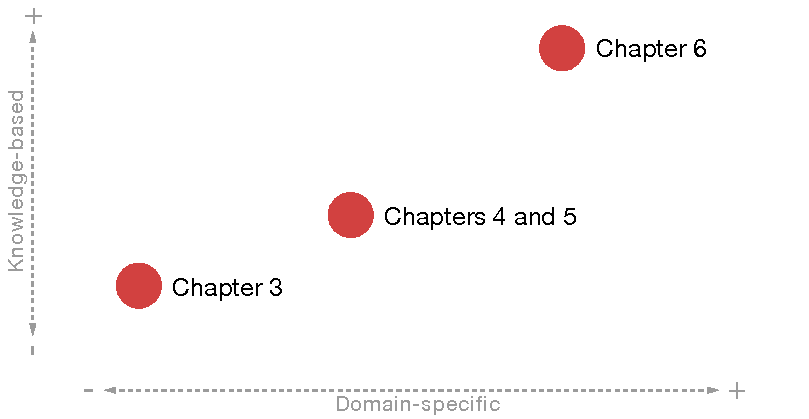
\includegraphics[width=0.8\textwidth]{ch01_introduction/pics/chapters_diagram}
  \caption[Conceptual organisation of Chapters~\ref{sec:general} to~\ref{sec:ontology}]{Conceptual organisation of Chapters~\ref{sec:general} to~\ref{sec:ontology} of this thesis according to the characteristics of the tag recommendation methods described therein.}
  \label{fig:chapters_diagram}
\end{figure}

In Chapter~\ref{sec:general}, we describe a generic scheme for folksonomy-based tag recommendation. This consists of three steps for which we provide several strategies.
By combining these alternative strategies, we define several tag recommendation methods. These methods are systematically evaluated and compared to other state of the art folksonomy-based tag recommendation methods through a tag prediction task and using data from Freesound and Flickr. 
The goal of this chapter is, on the one hand, the definition of a common scheme and conceptualisation of the tag recommendation task that will be used in in subsequent chapters.
On the other hand, in this chapter we compare our proposed methods with state of the art alternatives.
Our evaluation shows that the proposed methods can successfully generate tag recommendations both in the image and audio domains, performing significantly above the other evaluated methods.

Chapter~\ref{sec:class} extends the best performing tag recommendation method presented in the previous chapter by including a new step in which the resources being annotated are automatically classified into five broad audio categories.
Using this classification, the system is able to tailor tag recommendations to every particular audio category.
The recommendation system described in this chapter takes advantage of simple knowledge, specific to the audio domain, embedded in the audio classifier.
It is evaluated against the best performing method presented in the previous chapter, and against two random baselines through an online user experiment with 190 participants carried out in the context of Freesound. Furthermore, a complementary evaluation is also performed following the same evaluation strategy as in the previous chapter. The objective of this chapter is to evaluate whether the introduction of simple domain-specific knowledge in the form of resource categories can improve the usefulness of the tag recommendations generated by our previous method. 
Results show that the extended recommendation method represents an improvement over the previous method.%, according to both user-based and prediction-based evaluations.

In Chapter~\ref{sec:impact}, we analyse the impact of the tag recommendation method described in the previous chapter after we introduced it in the real-world tagging system of Freesound.
The goal of this chapter is the assessment of several hypotheses that have been made in the tagging literature regarding the impact that tag recommendation methods could have on the folksonomies of tagging systems. 
To the best of our knowledge, this is the first time that such an analysis has been made.
For this, we propose a series of evaluation metrics to illustrate different aspects of these hypotheses, and compute such metrics over data gathered during three months of activity after the deployment of the tag recommendation system, and over data from the previous two and a half years.
The analysis reveals that the tag recommendation system effectively contributes to the vocabulary convergence of the Freesound folksonomy, partially contributes to an improvement of annotation quality, but does not seem to significantly reduce the cost of the tagging process.

In Chapter~\ref{sec:ontology}, we explore a new perspective for folksonomy-based tag recommendation in which we introduce more domain-specific knowledge modelled with an ontology. We describe an ontology which embeds information about audio categories, tag categories and their relations. We describe a prototype for a tag recommendation system which makes extensive use of the ontology to provide the recommendations and evaluate it with two online experiments. 
Our particular goal in this chapter is to explore whether we can build tag recommendation systems that, by taking more advantage of domain-specific and structured knowledge, can help users in generating better quality resource annotations. Results show that using the tag recommendation prototype we describe, users can effectively generate better quality resource annotations. Nevertheless, we also observe that several improvements should be made before deploying such a system in a real-world scenario.

At the end of each chapter, we include a focused discussion about the relevant results and conclusions.
We conclude this thesis in Chapter~\ref{sec:conclusion} with a summary of our work, our main conclusions, and with a discussion about future perspectives of sound sharing, tag recommendation, and tagging systems in general.